\documentclass[a4paper]{article}
\usepackage[a4paper,%
    text={180mm, 260mm},%
    left=15mm, top=15mm]{geometry}
\usepackage[utf8]{inputenc}
\usepackage{cmap}
\usepackage[english, russian]{babel}
\usepackage{indentfirst}
\usepackage{amssymb}
\usepackage{amsmath}
\usepackage{mathtools}
\usepackage{tcolorbox}
\usepackage{graphicx}
\graphicspath{ {./figures} }

\begin{document}
\section*{Гиперболические ф-ии}

\[
    \ch z = \frac{e^{z}+e^{-z}}{2}, \quad \sh z = \frac{e^{z}-e^{-z}}{2}  
\]
\[
    \cos z = ch(iz) \quad (\ch z)' = \sh z
\]
\[
    \ch^2 z - \sh^2 z = 1
\]
\[
    \th z = \frac{\sh z}{\ch z} 
\]
\section*{Обратные тригонометрические ф-ии}

\begin{equation*}
    \begin{aligned}
        \cos z = 5\\
        z = Arccos 5 \\
        \frac{e^{iz} + e^{-iz}}{2} = 5 \; | \; 2 e^{iz}\\
        e^{2iz} - 10 e^{iz} + 1 = 0 \\
        e^{iz}= t \\
        t^2 - 10 t + 1 = 0\\
        t_{1,2}  = 5 \pm \sqrt{25-1} \\
        t_1 = 5 - \sqrt{24} \\
        t_2 = 5 + \sqrt{24} \\
        e^{iz} = 5 - \sqrt{24} \\
        iz = Ln(& - \sqrt{24})\\
        iz = \ln (5 - \sqrt{24}) + 2k \pi i, \; k \in \mathbb{Z}\\
        z = -i \cdot \ln(5-\sqrt{24}) + 2k \pi\\
        w = ? \quad z = \cos w\\
        e^{iw} = t, \; t \neq 0 \\
        z = \frac{t + t^{-1}}{2} \; | \; \cdot 2 \\
        t^{2} - 2zt + 1 = 0 \\
        t_{1,2}= z \pm \sqrt{z^2 - 1} \\
        e^{iw} = z \pm \sqrt{z^2 - 1} \\
        iw = Ln(z \pm \sqrt{z^2 - 1} \\
        w \equiv Ln(z \pm \sqrt{z^2 -1} \\
        w \equiv Arccos z = \frac{1}{i} Ln(z + \sqrt{z^2 -1} ) \; z = \pm 1\\
    \end{aligned}
\end{equation*}

\section*{\centering Конформные отображения}

\[
    w \equiv \Phi(z) = u + iv
\]
\begin{tcolorbox}
    \underline{Th1} $ w = \Phi(z)  $ непр. в обл. Д и однолистная на $ M = \Phi(D) \implies
    M$ - область

    \underline{Th2} при условии теоремы 1, то образом границы область D является
    граница области M (однако однозначности на границе может не сохранится) 

\end{tcolorbox}

\section*{\centering Геометрический смысл производной ф-ии}

\[
    w = f(z) - \text{ регулярна в т. z }
\]
И будем предпологать:
\[
    f'(z) \neq 0
\]

\begin{figure}[h!]
    \centering
    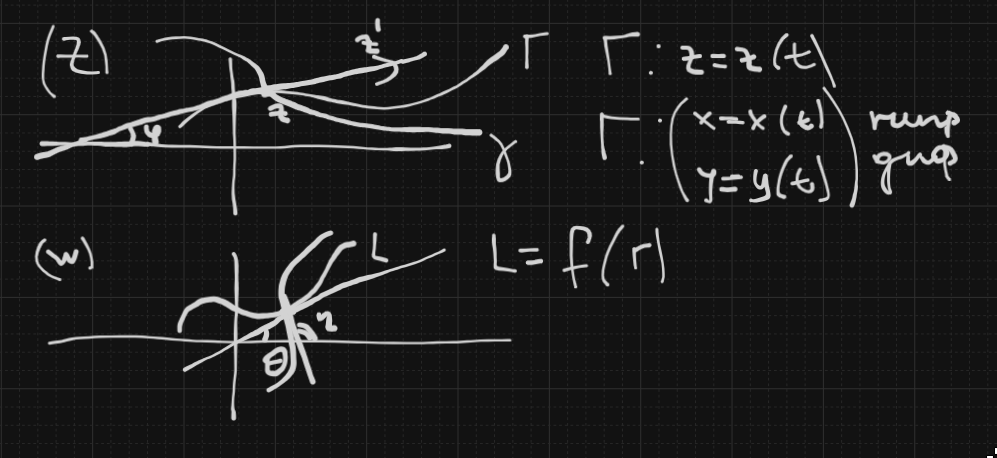
\includegraphics[width=0.95\textwidth]{tfpc-1-10-pic1.png}
    \caption{Геом. смысл производной}
\end{figure}

\begin{figure}[h!]
    \centering
    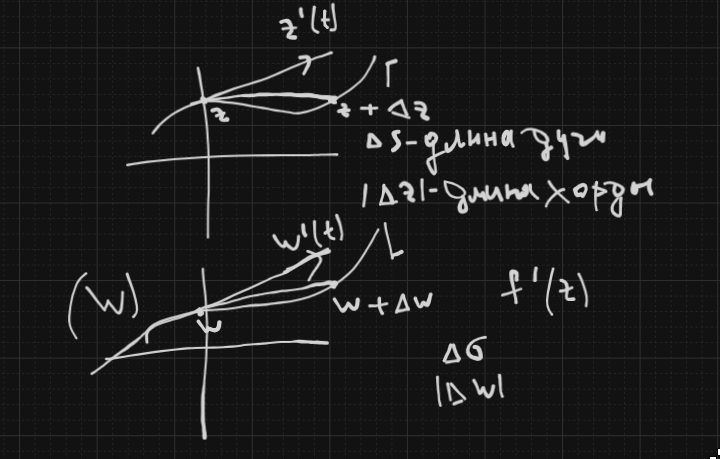
\includegraphics[width=0.95\textwidth]{tfcp-fig1-part2.png}
    \caption{Продолжения рис1}
\end{figure}

\[
    f'(z) = \rho \cdot e^{i\alpha}, \quad \rho = |f'(z)| \quad \alpha = \arg f'(z)
\]

\[
    \Gamma \text{ - гладкая } \implies (x'(t))^2 + (y'(t))^2 \neq 0
\]

\[
    z'(t) = x'(t) + iy'(t) \neq 0
\]
\[
    \phi = \arg z'(t)
\]
\[
    L: \; w \equiv w(t) = f(z(t))
\]

\[
    w'(t) = f'(z) \cdot z'(t) \neq 0
\]
\[
    \theta = \arg w'(t)
\]
\[
    \arg w'(t) = \arg f'(z) + \arg z'(t)
\]
\[
    \alpha = \theta - \phi
\]

\underline{Вывод 1} $ f'(z) \neq 0, \; \alpha = \arg f'(z) \implies $ Аргумент $ f'(z) $ 
равен углу поворота касательной в точке z при отображении $ w = f(z) $ (геометрический
смысл аргумента производной)

Рассмотрим через точку z другую гладкую кривую $ \gamma $ \\
\[
    \gamma: \arg\gamma = \psi \quad l = f(\gamma): \eta \implies \dots 
    \; \alpha = \eta - \psi
\]
\[
    \alpha = \theta - \phi = \eta - \psi
\]
\[
    \theta - \eta = \phi - \psi
\]

\underline{Вывод 2} $ f'(z) \neq 0 \implies $ при отображении $ w = f(z) $ 
угол между $ \Gamma, \; \gamma $ проход. через точку z равен по величине и 
по направлению отсчёта углу между образами этих кривых L и l в соответствующей точке w
(свойство консерватизма углов)

\[
    f'(z) = \lim_{\Delta z \to 0} \frac{\Delta w}{\Delta z} 
\]
\[
    |f'(z)| = \lim_{\Delta z \to 0} \left|\frac{\Delta w}{\Delta z} \right|
\]
\[
    |f'(z)| = \lim_{\Delta s \to 0} \frac{\Delta \sigma}{\Delta s} 
\]

\underline{Вывод 3} При отображении $ w = f(z) $ модуль производной $ \rho = |f'(z)| $ 
- коэф-т линейного расстяжения кривой Г в точке z (коэф. расстяжения малых векторов
выпущенных из точки z)

\underline{Def 1} Отбражение $ w = f(z) $ , при котором в данной точке z имеет место:\\
1) Консерватизм углов \\
2) Постоянство искажения линейного масштаба\\
Называется \underline{конформным или конформным первого рода} отображением

\underline{Def 2} $ w = f(z) $ области D на область $ G = f(D) $ называется конф., если
оно конформно в любой точке $ z \in D $ и однолистно

\underline{Def 3} Если при отображении углы между кривыми сохраняются по величине, но
направление отсчёта меняется на противоположное, то такое отображение называется
конформным 2-го рода

\begin{tcolorbox}
    \underline{Th} $ w = f(z) \in H(D) $ однозначная и аналитическая
    является конформной в каждой точке z, где $ f'(z) \neq 0 $ 
\end{tcolorbox}

\begin{tcolorbox}
    \underline{Th Римана} \\
    1) односвязная отсносительно расширенной комплексной плоскости $ \overline{\mathbb{C}} $
    граница которой содержит более одной точки можно конформно отобразить
    на единичный круг $ |w| < 1 $ \\
    2) нельзя конформно отобразить на единичный круг плоскость с одной выколотой
    точкой, а также многосвязную область на односвязную
\end{tcolorbox}

\section*{\centering Теоремы единственности конформного отображения}
\begin{tcolorbox}
    1) заданную точку $ z_0 \in D $ и направление $ \phi $ отобразить в заданную 
    точку $ w_0 \in G $ и направление $ \theta $ в этой точке

    2) заданную внутренную точку $ z_0 \in D $ и граничную точку $ z_1 \in \partial D $ 
    отобразить в заданную внутреннюю точку $ w \in G $ и заданную граничкую
    $ w_1 \in \partial G $ 

    3) три заданные граничные точки $ z_1, z_2, z_3 \in \partial D $ отобразить
    в три заданные граничные точки $ w_1, w_2, w_3 \in \partial G $ при сохранении
    обхода по границе $ w_1 = f(z_1), \; w_2 = f(z_2), \; w_3 = f(z_3) $ 
\end{tcolorbox}

\section*{\centering Линейное отображение}
\end{document}
